\section{Simulator architecture}\label{sec:sim_architecture}

\subsection{ROS}

As mentioned above, the SnakeSIM simulator is based in and run from ROS, which is a set of open source software libraries and tools designed to build robot applications.
The use of nodes ensures the modular architecture of ROS. A node is an independent part of the program that has a specific computation task. More concretely, it is an executable file from a ROS package. An example of this is the position controller node or the collisions node, detecting and reporting collisions. The nodes are in this project programmed using C++. Another supported alternative is Python. The modular architecture of ROS even allows for the nodes to be developed with different programming languages without any complications.

Even though the nodes are able to run independently, they might need data from other nodes to make useful computations. The nodes therefore communicate with each other with the use of topics. A topic is simply a set of variables that can be continuously updated by a node. Updating these variables are referred to as publishing to the topic. At the same time other nodes may read the values posted on this topic. This is done by subscribing to the topic. There is no limit to how many nodes can publish and subscribe to a specific topic. A visualization of an example of this message passing system is presented in Figure \ref{fig:nodesntopics}.

\begin{figure}
    \centering
    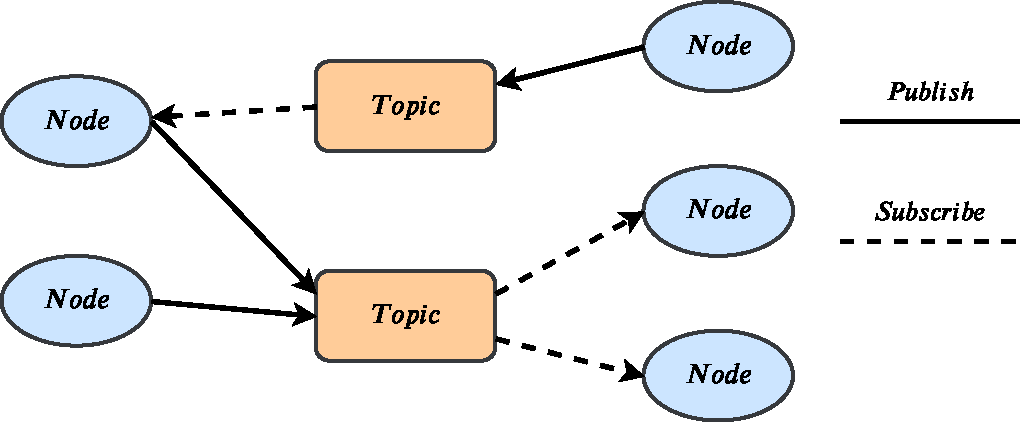
\includegraphics[width=0.9\textwidth]{figures/simulator/nodesntopics.pdf}
    \caption{Message passing system in ROS}
    \label{fig:nodesntopics}
\end{figure}

The nodes are able to find each other and communicate thanks to the ROS master. It registers all the 
running nodes and tracks topic publishing and subscriptions.

\subsection{Gazebo}

The ROS-based program is set up to launch the Gazebo 3D physics simulator. Gazebo is adapted to accurately simulate the snake robot in the desired environment with obstacles. All simulated objects, meaning the snake robot and the obstacles, have attributes like mass and velocity. This allows for realistic behaviour when interaction and collisions occur. The configuration of the simulated snake robot and obstacles is implemented according to the Universal Robotic Description Format (URDF) \cite{urdfWeb}. This is an XML-based file format used to describe elements like links, joints, sensors and actuators and how these elements connect to each other.

The added sensors are able to communicate properties like forces, torques, contact positions, etc. These properties, as well as all physical variables, are reported back to ROS by Gazebo.
At the same time, Gazebo subscribes to information from the ROS controller nodes sending joint motor torque commands for the snake robot. The physics engine is then able to use all this information to enable Gazebo to show a realistic resulting movement. It is also possible to move and influence the simulated objects directly through the graphical user interface (GUI) provided by Gazebo (see Figure \ref{fig:gazebo_gui}).

\begin{figure}
    \centering
    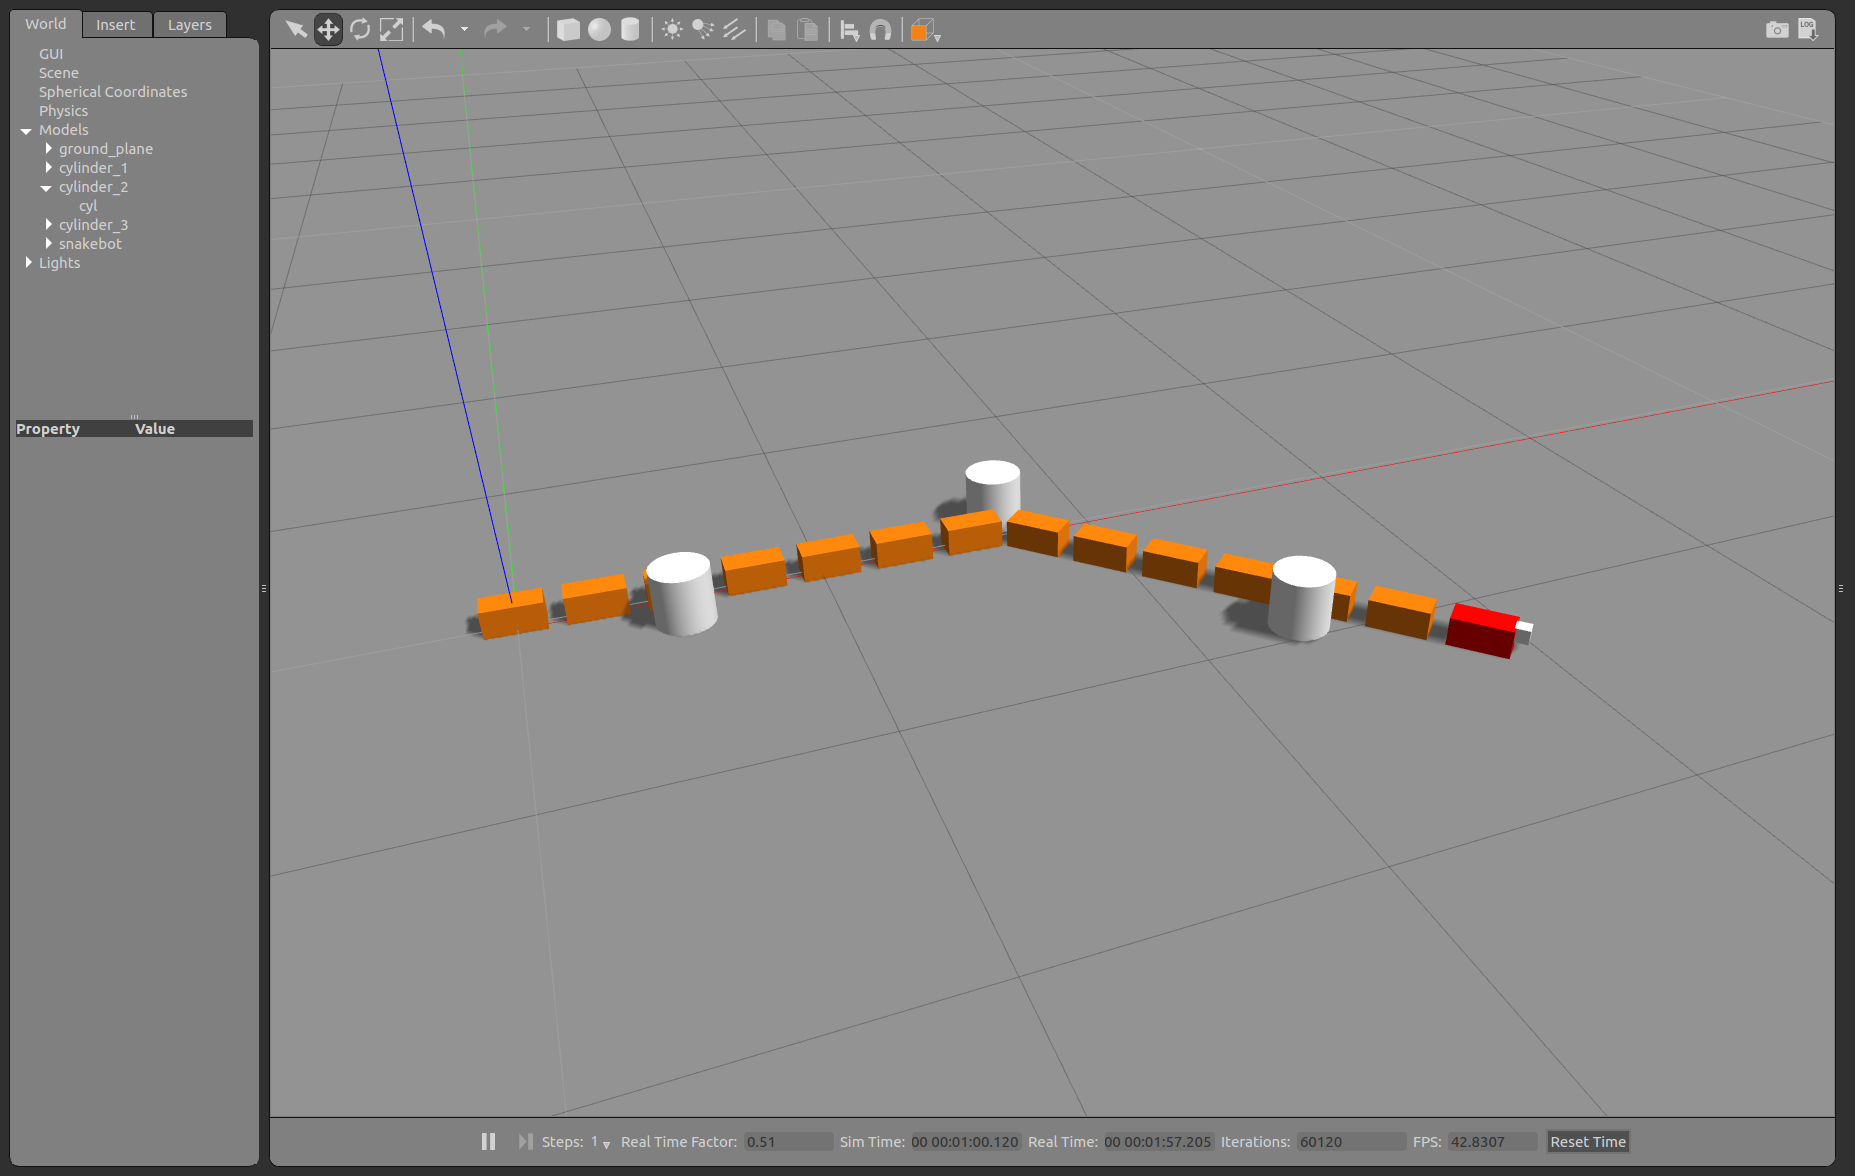
\includegraphics[width=1\textwidth]{figures/simulator/gazebo_gen_screen.png}
    \caption{Gazebo graphical user interface}
    \label{fig:gazebo_gui}
\end{figure}